\section{Online News}\label{sec:OnlineNewsChap}

O segundo dataset escolhido foi o Online News. Este conjunto de dados sumariza várias características de artigos publicados online no Mashable, durante um período de dois anos. A data da recolha é 8 de janeiro de 2015. Este conjunto de dados tem mais de 34.600 registos com 61 atributos cada. Não tem valores nulos, contudo existem valores não classificados. O objetivo primordial do conjunto de dados é estimar o número de partilhas de um artigo.

\subsection{Objetivos do estudo}

Aquando da escolha deste conjunto de dados uma das coisas que foi imediatamente referenciada pelo Professor foi a presença de grande número de atributos. Foi esse o nosso ponto de partida para o estudo deste conjunto de dados. Tentar perceber quais os atributos que realmente iriam contribuir para o estudo em causa e quais aqueles que poderiam ser descartados. \newline
O segundo ponto do estudo será perceber quais as características principais que tornam um artigo mais partilhado ou menos partilhado e a forma como os próprios jornalistas podem usar técnicas para melhorar a performance social do artigo/notícia.

\subsection{Atributos do conjunto de dados}

De seguida listam-se os atributos originais do conjunto de dados e a sua descrição.

\begin{table}
\centering
\label{my-label2}
\resizebox{\textwidth}{!}{\begin{tabular}{|l|l|l|}
Atributo                         & Descrição                                                                                     & Tipo           \\ \hline
url                              & Endereço do artigo, atributo não preditivo                                                    & String         \\ \hline
timedelta                        & \makecell{Tempo entre a publicação do artigo\\ e a aquisição do conjunto de dados, atributo não preditivo} & Valor numérico \\ \hline
n\_tokens\_title                 & Número de palavras no título                                                                  & Valor numérico \\ \hline
n\_tokens\_content               & Número de palavras do artigo                                                                  & Valor numérico \\ \hline
n\_unique\_tokens                & Percentagem de palavras únicas no artigo                                                      & Valor numérico \\ \hline
n\_non\_stop\_unique\_tokens     & Percentagem de "palavras vazias" no artigo                                                    & Valor numérico \\ \hline
num\_hrefs                       & Número de links externos                                                                      & Valor numérico \\ \hline
num\_self\_hrefs                 & Número de links para outros artigos do Mashable                                               & Valor numérico \\ \hline
num\_imgs                        & Número de imagens                                                                             & Valor numérico \\ \hline
num\_videos                      & Número de vídeos                                                                              & Valor numérico \\ \hline
average\_token\_length           & Média de tamanho das palavras no artigo                                                       & Valor numérico \\ \hline
num\_keywords                    & Número de palavras-chave                                                                      & Valor numérico \\ \hline
data\_channel\_is\_lifestyle     & Da categoria Lifestyle                                                                        & Boleano        \\ \hline
data\_channel\_is\_entertainment & Da categoria Entretenimento                                                                   & Boleano        \\ \hline
data\_channel\_is\_bus           & Da categoria Business                                                                         & Boleano        \\ \hline
data\_channel\_is\_socmed        & Da categoria Social Media                                                                     & Boleano        \\ \hline
data\_channel\_is\_tech          & Da categoria Tecnologia                                                                       & Boleano        \\ \hline
data\_channel\_is\_world         & Da categoria Mundo                                                                            & Boleano        \\ \hline
kw\_min\_min                     & Mínimo de partilhas da pior palavra-chave                                                     & Valor numérico \\ \hline
kw\_max\_min                     & Máximo de partilhas da pior palavra-chave                                                     & Valor numérico \\ \hline
kw\_avg\_min                     & Média de partilhas da pior palavra-chave                                                      & Valor numérico \\ \hline
kw\_min\_max                     & Mínimo de partilhas da melhor palavra-chave                                                   & Valor numérico \\ \hline
kw\_max\_max                     & Máximo de partilhas da melhor palavra-chave                                                   & Valor numérico \\ \hline
kw\_avg\_max                     & Média de partilhas da melhor palavra-chave                                                    & Valor numérico \\ \hline
kw\_min\_avg                     & Mínimo de partilhas da palavra-chave média                                                    & Valor numérico \\ \hline
kw\_max\_avg                     & Máximo de partilhas da palavra-chave média                                                    & Valor numérico \\ \hline
kw\_avg\_avg                     & Média de partilhas da palavra-chave média                                                     & Valor numérico \\ \hline
self\_reference\_min\_shares     & Mínimo de partilhas dos artigos próprios referenciados                                        & Valor numérico \\ \hline
self\_reference\_max\_shares     & Máximo de partilhas dos artigos próprios referenciados                                        & Valor numérico \\ \hline
self\_reference\_avg\_sharess    & Média de partilhas dos artigos próprios referenciados                                         & Valor numérico \\ \hline
weekday\_is\_monday              & Publicado há segunda                                                                          & Boleano        \\ \hline
weekday\_is\_tuesday             & Publicado há terça                                                                            & Boleano        \\ \hline
weekday\_is\_wednesday           & Publicado há quarta                                                                           & Boleano        \\ \hline
weekday\_is\_thursday            & Publicado há quinta                                                                           & Boleano        \\ \hline
weekday\_is\_friday              & Publicado há sexta                                                                            & Boleano        \\ \hline
weekday\_is\_saturday            & Publicado há sábado                                                                           & Boleano        \\ \hline
weekday\_is\_sunday              & Publicado há domingo                                                                          & Boleano        \\ \hline
is\_weekend                      & Publicado ao fim-de-semana                                                                    & Boleano        \\ \hline
LDA\_00                          & Proximidade ao tópico 0 do LDA                                                                & Valor numérico \\ \hline
LDA\_01                          & Proximidade ao tópico 1 do LDA                                                                & Valor numérico \\ \hline
LDA\_02                          & Proximidade ao tópico 2 do LDA                                                                & Valor numérico \\ \hline
LDA\_03                          & Proximidade ao tópico 3 do LDA                                                                & Valor numérico \\ \hline
LDA\_04                          & Proximidade ao tópico 4 do LDA                                                                & Valor numérico \\ \hline
global\_subjectivity             & Subjetividade global do artigo                                                                & Valor numérico \\ \hline
global\_sentiment\_polarity      & Polaridade do sentimento do texto                                                             & Valor numérico \\ \hline
global\_rate\_positive\_words    & Percentagem de palavras positivas no artigo                                                   & Valor numérico \\ \hline
global\_rate\_negative\_words    & Percentagem de palavras negativas no artigo                                                   & Valor numérico \\ \hline
rate\_positive\_words            & Rácio de palavras positivas e neutras                                                         & Valor numérico \\ \hline
rate\_negative\_words            & Rácio de palavras negativas e neutras                                                         & Valor numérico \\ \hline
avg\_positive\_polarity          & Média de polaridade das palavras positivas                                                    & Valor numérico \\ \hline
min\_positive\_polarity          & Mínimo de polaridade das palavras positivas                                                   & Valor numérico \\ \hline
max\_positive\_polarity          & Máximo de polaridade das palavras positivas                                                   & Valor numérico \\ \hline
avg\_negative\_polarity          & Média de polaridade das palavras negativas                                                    & Valor numérico \\ \hline
min\_negative\_polarity          & Mínimo de polaridade das palavras negativas                                                   & Valor numérico \\ \hline
max\_negative\_polarity          & Máximo de polaridade das palavras negativas                                                   & Valor numérico \\ \hline
title\_subjectivity              & Subjetividade do título                                                                       & Valor numérico \\ \hline
title\_sentiment\_polarity       & Polaridade do sentimento do título                                                            & Valor numérico \\ \hline
abs\_title\_subjectivity         & Grau de subjetividade global do título                                                        & Valor numérico \\ \hline
abs\_title\_sentiment\_polarity  & Grau de polaridade do título                                                                  & Valor numérico \\ \hline
shares                           & Número de partilhas                                                                           & Valor numérico \\ \hline
\end{tabular}}
\end{table}
\newpage
Pela primeira análise aos atributos conseguimos facilmente perceber que o conjunto de dados é de bastante valor um vez que temos vários atributos de valor numérico e grande quantidade de atributos e informação. A tabela seguinte relaciona os atributos entre si:

\begin{figure}[H]
    \centering
    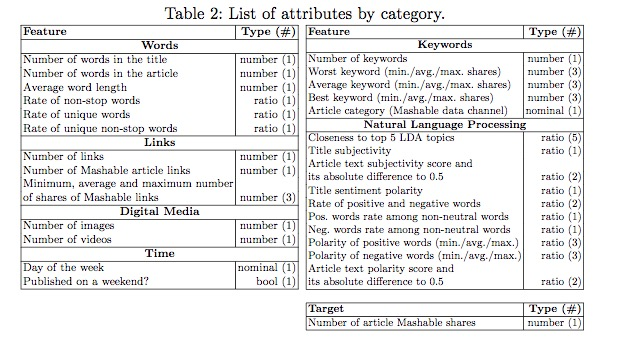
\includegraphics[scale=0.5]{tex/img/img1o.jpg}
    \caption{Atributos por categoria}
    \label{fig:atributosOn}
\end{figure}


\subsection{LDA}

Um dos atributos que nos chamou mais à atenção, até porque não entendemos o que realmente significa foi o LDA (os 4 atributos relacionados com este tópico). Foi então necessário investigar o que significava. O LDA, Latent Dirichlet Allocation ou alocação latente de Dirichlet é um modelo estatístico generativo que permite explicar conjunto de observações através de grupos não observados, que explicam o porquê de algumas partes dos dados serem semelhantes.
Por exemplo, à semelhança do modelo mostrado de seguida, se as observações são palavras adquiridas de vários documentos, isso deriva que cada documento é uma mistura de um pequeno número de tópicos e que a criação de cada palavra é atribuível a um dos tópicos do documento.\newline
Assim, este atributo mede a proximidade do artigo a cada um dos cinco tópicos principais do texto identificados pelo algoritmo.

\begin{figure}[H]
    \centering
    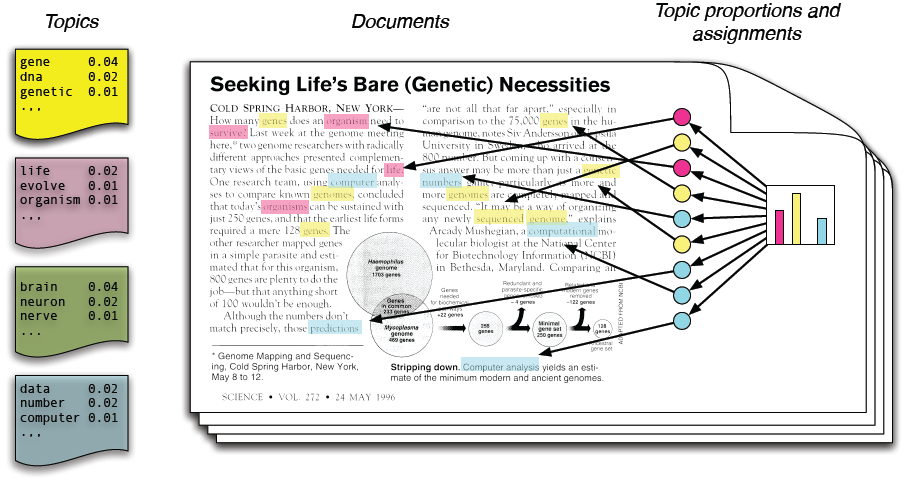
\includegraphics[scale=0.3]{tex/img/lda.png}
    \caption{O algoritmo LDA}
    \label{fig:LDAOn}
\end{figure}


\subsection{Preparação do conjunto}

O primeiro ponto para a preparação do conjunto foi remover alguns atributos \"triviais\". Os vários atributos data channel e date of publication foram convertidos em apenas dois com as seguintes associações:


\begin{table}[]
\centering
\label{my-labelOn}
\caption{Data Channel}
\begin{tabular}{|l|l|}
\hline
0 & Lifestyle     \\ \hline
1 & Entertainment \\ \hline
2 & Business      \\ \hline
3 & Social Media  \\ \hline
4 & Technology    \\ \hline
5 & World         \\ \hline
6 & Other         \\ \hline
\end{tabular}
\end{table}

\begin{table}[]
\centering
\label{my-labelOn2}
\caption{Date of Publication}
\begin{tabular}{|l|l|}
\hline
0 & segunda-feira \\ \hline
1 & terça-feira   \\ \hline
2 & quarta-feira  \\ \hline
3 & quinta-feira  \\ \hline
4 & sexta-feira   \\ \hline
5 & sábado        \\ \hline
6 & domingo       \\ \hline
\end{tabular}
\end{table}

O passo seguinte será perceber quais os atributos \"descartáveis\" e aqueles que mais contribuem para calcular o quão partilhável é um artigo. Contudo, neste aspeto já recorremos a algoritmos de Seleção de Atributos.

\subsection{Seleção de Atributos}

Como já foi indicado o primeiro passo foi selecionar os atributos que mais contribuem para a Class. Não só porque o conjunto de dados tinha um grande volume de atributos como também para perceber quais desses contribuem realmente para as partilhas do artigo e aqueles que menos contribuem. Para isto foi utilizam o algoritmo CorrelationAttributeEval que avalia o valor de um atributo medindo a correlação entre o atributo e a classe (número de partilhas). Este algoritmo precisa também de um método de pesquisa e o mais indicado e com o qual obtivemos melhores resultados foi o Ranker que classifica os atributos através das suas avaliações individuais.

\begin{figure}[H]
    \centering
    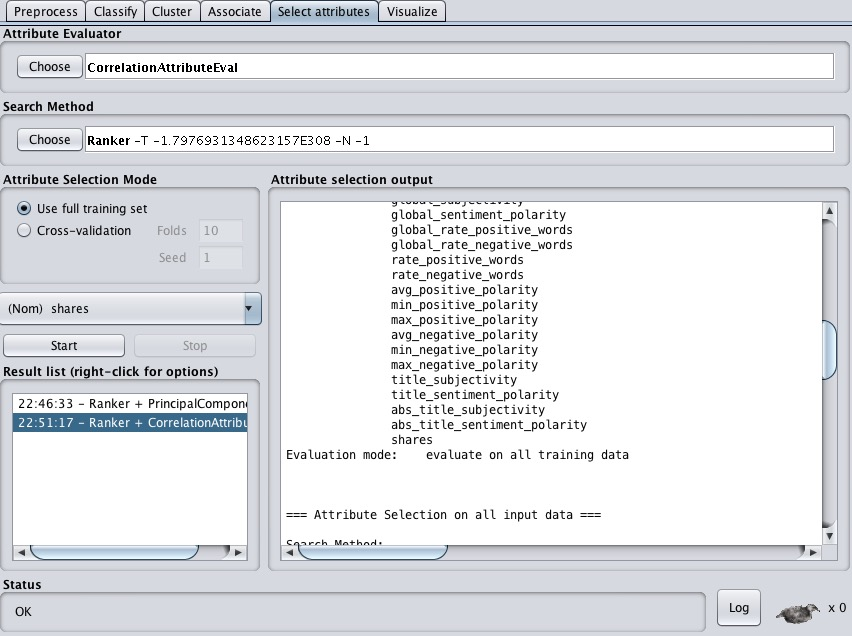
\includegraphics[scale=0.4]{tex/img/img2o.jpg}
    \caption{Configuração da Seleção de Atributos}
    \label{fig:SaOn}
\end{figure}
\newpage
\begin{lstlisting}[breaklines,frame=single]

=== Attribute Selection on all input data ===

Search Method:
  Attribute ranking.

Attribute Evaluator (supervised, Class (nominal): 47  shares):
  Correlation Ranking Filter
Ranked attributes:
 0.0163    28  LDA\_02
 0.01623   21  kw\_avg\_avg
 0.01259   11  num\_keywords
 0.01241   29  LDA\_03
 0.01208   12 data\_channel
 0.01205   30  LDA\_04
 0.01085   32  global\_sentiment\_polarity
 0.01081   36  rate\_negative\_words
 0.01043   26  LDA\_00
 0.0098    33  global\_rate\_positive\_words
 0.00962   20  kw\_max\_avg
 0.00935    6  num\_hrefs
 0.00912   27  LDA\_01
 0.00889    8  num\_imgs
 0.00879   19  kw\_min\_avg
 0.0084    43  title\_subjectivity
 0.00838   35  rate\_positive\_words
 0.00835   31  global\_subjectivity
 0.00785   46  abs\_title\_sentiment\_polarity
 0.00765   18  kw\_avg\_max
 0.00731   44  title\_sentiment\_polarity
 0.00697   10  average\_token\_length
 0.00688   38  min\_positive\_polarity
 0.00673   34  global\_rate\_negative\_words
 0.00668    7  num\_self\_hrefs
 0.0066    39  max\_positive\_polarity
 0.00631   23  self\_reference\_max\_shares
 0.00613   25 date\_publication
 0.00611   24  self\_reference\_avg\_sharess
 0.00609   40  avg\_negative\_polarity
 0.00606   41  min\_negative\_polarity
 0.00585    2  n\_tokens\_content
 0.00582   15  kw\_avg\_min
 0.00563   37  avg\_positive\_polarity
 0.00562   45  abs\_title\_subjectivity
 0.00559    1  n\_tokens\_title
 0.00538   14  kw\_max\_min
 0.00513    9  num\_videos
 0.00511   22  self\_reference\_min\_shares
 0.00489   42  max\_negative\_polarity
 0.00483   16  kw\_min\_max
 0.00319   17  kw\_max\_max
 0.00277   13  kw\_min\_min
 0.00107    3  n\_unique\_tokens
 0.00105    5  n\_non\_stop\_unique\_tokens
 0.00101    4  n\_non\_stop\_words

\end{lstlisting}

Como podemos ver pela seleção anterior quase todos os atributos contribuem para as partilhas, contudo atributos como o LDA\_02, o kw\_avg\_avg e o num\_keywords contribuem mais para o número de partilhas que um artigo vai ter do que por exemplo atributos como o n\_unique\_tokens e o n\_non\_stop\_words. Assim, esta lista serve como uma lista de prioridades a ter para um jornalista quando está a escrever um novo artigo.

\subsection{Análise dos Atributos}

De seguida analisam-se os atributos, referenciando quais os valores ótimos para se otimizar um artigo quanto ao número de partilhas.

\textbf{n\_tokens\_title}

\begin{figure}[H]
    \centering
    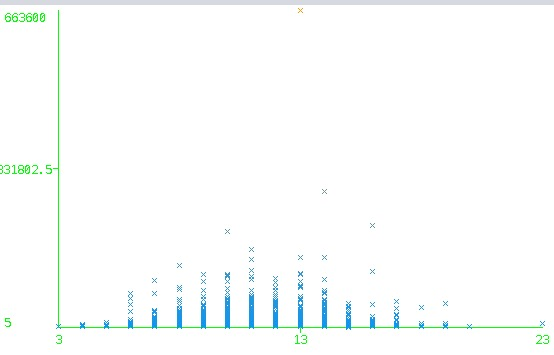
\includegraphics[scale=0.6]{tex/img/graph1.jpg}
    \caption{Relação entre o n\_tokens\_title e o número de partilhas}
    \label{fig:tokensTitles}
\end{figure}
Como podemos observar o número de palavras ótimo para o título é até 13 palavras.

\textbf{n\_tokens\_content}

\begin{figure}[H]
    \centering
    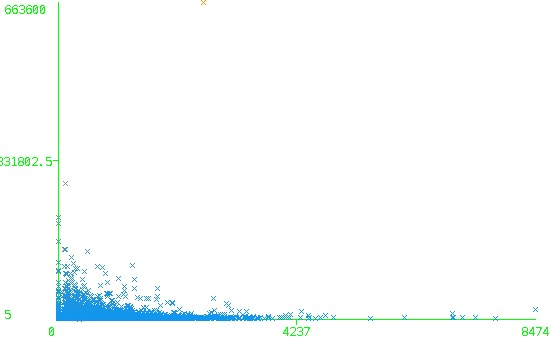
\includegraphics[scale=0.6]{tex/img/graph2.jpg}
    \caption{Relação entre o n\_tokens\_content e o número de partilhas}
    \label{fig:tokensTitles2}
\end{figure}

Artigos com menos palavras são mais partilhados. O ideal de palavras de um artigo é menos de 4237.

\textbf{num\_hrefs}

\begin{figure}[H]
    \centering
    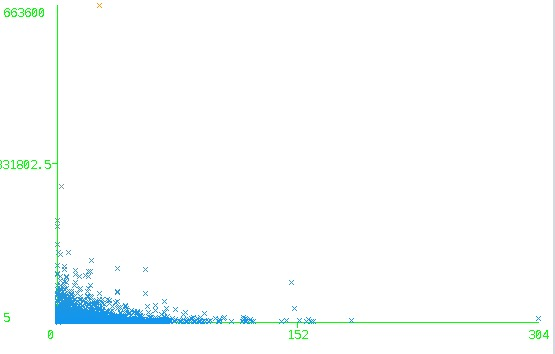
\includegraphics[scale=0.6]{tex/img/graph3.jpg}
    \caption{Relação entre o num\_hrefs e o número de partilhas}
    \label{fig:numHrefst}
\end{figure}

Artigos com menos links externos são mais partilhados.

\textbf{num\_self\_hrefs}

\begin{figure}[H]
    \centering
    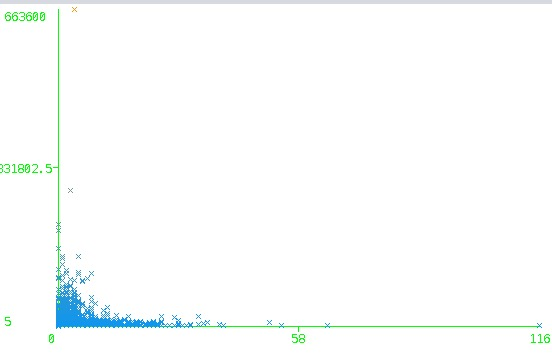
\includegraphics[scale=0.6]{tex/img/graph4.jpg}
    \caption{Relação entre o num\_self\_hrefs e o número de partilhas}
    \label{fig:numSelfHrefst}
\end{figure}

Artigos com menos links internos são mais partilhados.

\textbf{num\_imgs}

\begin{figure}[H]
    \centering
    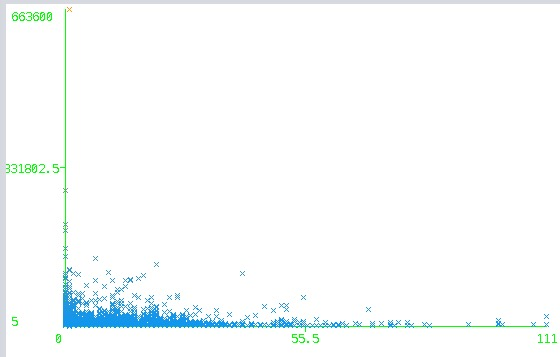
\includegraphics[scale=0.6]{tex/img/graph5.jpg}
    \caption{Relação entre o num\_imgs e o número de partilhas}
    \label{fig:numImgs}
\end{figure}

Um artigo deve ter menos de 55 imagens.

\textbf{n\_keywords}

\begin{figure}[H]
    \centering
    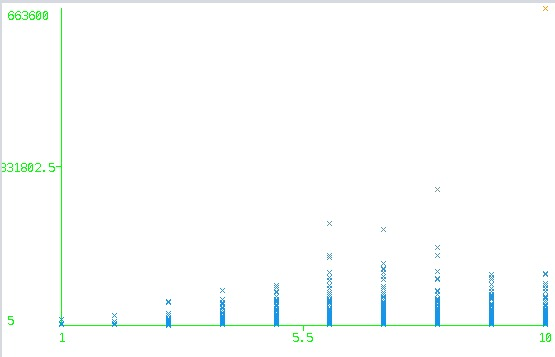
\includegraphics[scale=0.6]{tex/img/graph6.jpg}
    \caption{Relação entre o n\_keywords e o número de partilhas}
    \label{fig:nKeywords}
\end{figure}

O artigo deverá ter mais de 5.5 keywords e menos de 10.

\textbf{data\_channel}

\begin{figure}[H]
    \centering
    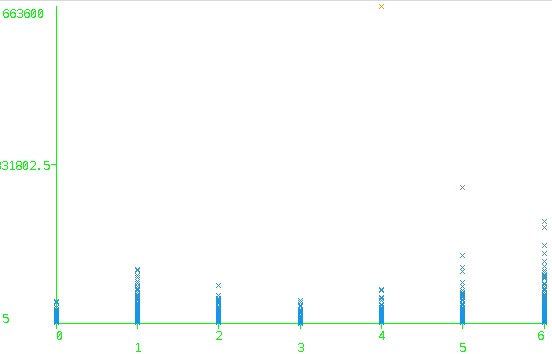
\includegraphics[scale=0.6]{tex/img/graph7.jpg}
    \caption{Relação entre o data\_channel e o número de partilhas}
    \label{fig:dataChannel1}
\end{figure}

Artigos de World, Other e Entertainment são mais partilhados.

\textbf{data\_channel}

\begin{figure}[H]
    \centering
    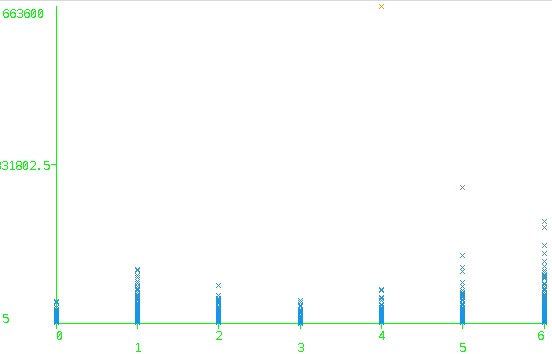
\includegraphics[scale=0.6]{tex/img/graph7.jpg}
    \caption{Relação entre o data\_channel e o número de partilhas}
    \label{fig:dataChannel2}
\end{figure}

Artigos de World, Other e Entertainment são mais partilhados.


\textbf{date\_publication}

\begin{figure}[H]
    \centering
    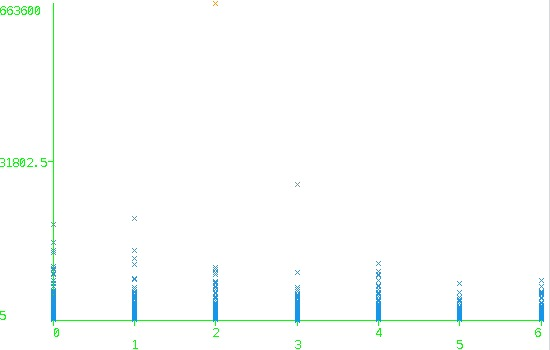
\includegraphics[scale=0.6]{tex/img/graph8.jpg}
    \caption{Relação entre o date\_publication e o número de partilhas}
    \label{fig:datePublication}
\end{figure}

Artigos publicados à segunda-feira e terça-feira são os mais publicados.


\subsection{Resultados e Recomendações}


Conseguimos assim obter os resultados pretendidos, de modo a obter noção das características um artigo deverá ter para ser mais viral, tornando-se mais partilhado pelos leitores. Da análise dos resultados obtidos tiramos ainda as seguintes recomendações, neste caso para o Mashable:

\begin{itemize}
  \item Publicar mais artigos durante a semana do que ao fim-de-semana;
  \item Publicar mais artigos sobre World e Entertainment e evitar artigos sobre Social Media e Business;
  \item Tentar focar e manter o artigo o mais possível perto do título;
  \item Publicar artigos com mais pequenos, com menos palavras;
  \item Títulos de artigos mais curtos resultam em mais partilhas;
\end{itemize}